
\documentclass{article} % Don't change this

\usepackage{tabularx} % extra features for tabular environment
\usepackage{amsmath}  % improve math presentation
\usepackage{graphicx} % takes care of graphic including machinery
\usepackage[margin=1.25in,letterpaper]{geometry} % decreases margins
\usepackage{cite} % takes care of citations
\usepackage{subfigure}
\usepackage{float}    % For tables and other floats
\usepackage[final]{hyperref} % adds hyper links inside the generated pdf file
\usepackage{listings}
\usepackage[framed,numbered,autolinebreaks,useliterate]{mcode}
\usepackage{lipsum}
\usepackage{appendix}
\usepackage{cite}
\hypersetup{
	colorlinks=true,       % false: boxed links; true: colored links
	linkcolor=blue,        % color of internal links
	citecolor=blue,        % color of links to bibliography
	filecolor=magenta,     % color of file links
	urlcolor=blue         
}
\newcommand{\blah}{blah blah blah \dots}



\setlength{\marginparwidth}{3.4cm}

% NEW COUNTERS
\newcounter{points}
\setcounter{points}{100}
\newcounter{spelling}
\newcounter{usage}
\newcounter{units}
\newcounter{other}
\newcounter{source}
\newcounter{concept}
\newcounter{missing}
\newcounter{math}

% COMMANDS
%\newcommand{\raisa}[2]{\colorbox{Yellow}{#1} \todo{#2}}
\newcommand{\arbitrary}[2]{\todo{#1 #2} \addtocounter{points}{#2} \addtocounter{other}{#2}}
\newcommand{\english}{\todo{LANGUAGE (-1)} \addtocounter{points}{-1}
\addtocounter{usage}{-1}}
\newcommand{\units}{\todo{UNITS (-1)} \addtocounter{points}{-1}
\addtocounter{units}{-1}}
\newcommand{\spelling}{\todo{SPELLING and GRAMMAR (-1)} \addtocounter{points}{-1}
\addtocounter{spelling}{-1}}
\newcommand{\source}{\todo{SOURCE(S) (-2)} \addtocounter{points}{-2}
\addtocounter{source}{-2}}
\newcommand{\concept}{\todo{CONCEPT (-2)} \addtocounter{points}{-2}
\addtocounter{concept}{-2}}
\newcommand{\missing}[2]{\todo{MISSING CONTENT (#1) #2} \addtocounter{points}{#1}
\addtocounter{missing}{#1}}
\newcommand{\maths}{\todo{MATH (-1)} \addtocounter{points}{-1}
\addtocounter{math}{-1}}

\newcommand{\summary}[1]{
\begin{mdframed}[nobreak=true]
\begin{minipage}{\textwidth}
\vspace{0.5cm}
\begin{center}
\Large{Grade Summary} \hrule 
\end{center} \vspace{0.5cm}
General Comments: #1

\vspace{0.5cm}
Possible Points \dotfill 100 \\
Points Lost (Spelling and Grammar) \dotfill \thespelling \\
Points Lost (Language) \dotfill \theusage \\
Points Lost (Units) \dotfill \theunits \\
Points Lost (Math) \dotfill \themath \\
Points Lost (Sources) \dotfill \thesource \\
Points Lost (Concept) \dotfill \theconcept \\
Points Lost (Missing Content) \dotfill \themissing \\
Other \dotfill \theother \\[0.5cm]
\begin{center}
\large{\textbf{Grade:} \fbox{\thepoints}}
\end{center}
\end{minipage}
\end{mdframed}}

%#########################################################

%To use symbols for footnotes
\renewcommand*{\thefootnote}{\fnsymbol{footnote}}
%To change footnotes back to numbers uncomment the following line
%\renewcommand*{\thefootnote}{\arabic{footnote}}

% Enable this command to adjust line spacing for inline math equations.
% \everymath{\displaystyle}

% _______ _____ _______ _      ______ 
%|__   __|_   _|__   __| |    |  ____|
%   | |    | |    | |  | |    | |__   
%   | |    | |    | |  | |    |  __|  
%   | |   _| |_   | |  | |____| |____ 
%   |_|  |_____|  |_|  |______|______|
%%%%%%%%%%%%%%%%%%%%%%%%%%%%%%%%%%%%%%%

\title{
\normalfont \normalsize 
\textsc{Rutgers University \\ 
Summer Research Program} \\
[10pt] 
\rule{\linewidth}{0.5pt} \\[6pt] 
\huge Preparation for GpyTorch Implementation  \\
\rule{\linewidth}{2pt}  \\[10pt]
}
\author{Han Liu}
\date{\normalsize \today}

\begin{document}

\maketitle



\section{Introduction}
In the process of training and predicting a gaussian process (GP), we need to get three quantities: the mean of predicted input, the log marginal likelihood function and its derivative. Their expressions are given as following:
\begin{equation}
u_{f|D}(\hat{x})=u(\hat{x})+k_{X\hat{x}}^{T}K^{-1}y
\end{equation}

\begin{equation}\label{eq1}
logp({y|K})=-\frac{1}{2}log((2\pi)^k|K|)-\frac{1}{2}y^T{K}^{-1}y
\end{equation}

\begin{equation}
\frac{\partial}{\partial \theta_j}logp(y|X,\theta)=\frac{1}{2}y^{T}K^{-1}\frac{\partial K}{\partial \theta_j}K^{-1}y-\frac{1}{2}tr(K^{-1}\frac{\partial K}{\partial \theta_j})
\end{equation}
These equation have three operations in common that dominate its time complexity: $K^{-1}y$, $log|K|$, $tr(K^{-1}\frac{\partial K}{\partial \theta_j})$. Before that, I use Cholesky decomposition of $K$ to compute all three quantities (see $GP\_code.py$), but it is very computational expensive, thus we need some parallel computional algorithm.\\
I think the innovative part of this paper is to use matrix-matrix multipy to combine three algorithms (Conjugate Gradient, Lancos Algorithm, Pivoted Cholesky Decomposition) together. The most important formula is as following:
\begin{equation}\label{equ1}
[u_0 \quad u_1 \quad ... \quad u_t]=K^{-1}[y \quad z_1 \quad ... \quad z_t]
\end{equation}
The whole algorithm flow chart can be seen in Figure \ref{fig1}. In the following section, I will implement all the three algorithms individually by MATLAB.


\section{The Pivoting Cholesky Decomposition}
In the process of implementing the pivoting cholesky decomposition, I found the algorithm I derived last week had some problems, so I have implemented it again. Specifically, we need to find $P^TKP=R^TR$ for symmetric positive matrix $K\in R^{n\times n}$, where $P$ is permutation matrix. Following the derivation of the pivoting cholesky decomposition in the paper, we need to use one propertiy of permutation matrix:
\begin{equation}
P^{-1}=P^{T}
\end{equation}
The mathematical details are given in appendix. Specifically, the whole algorithm should be as following:
 \begin{figure}[h]
	\begin{center}
		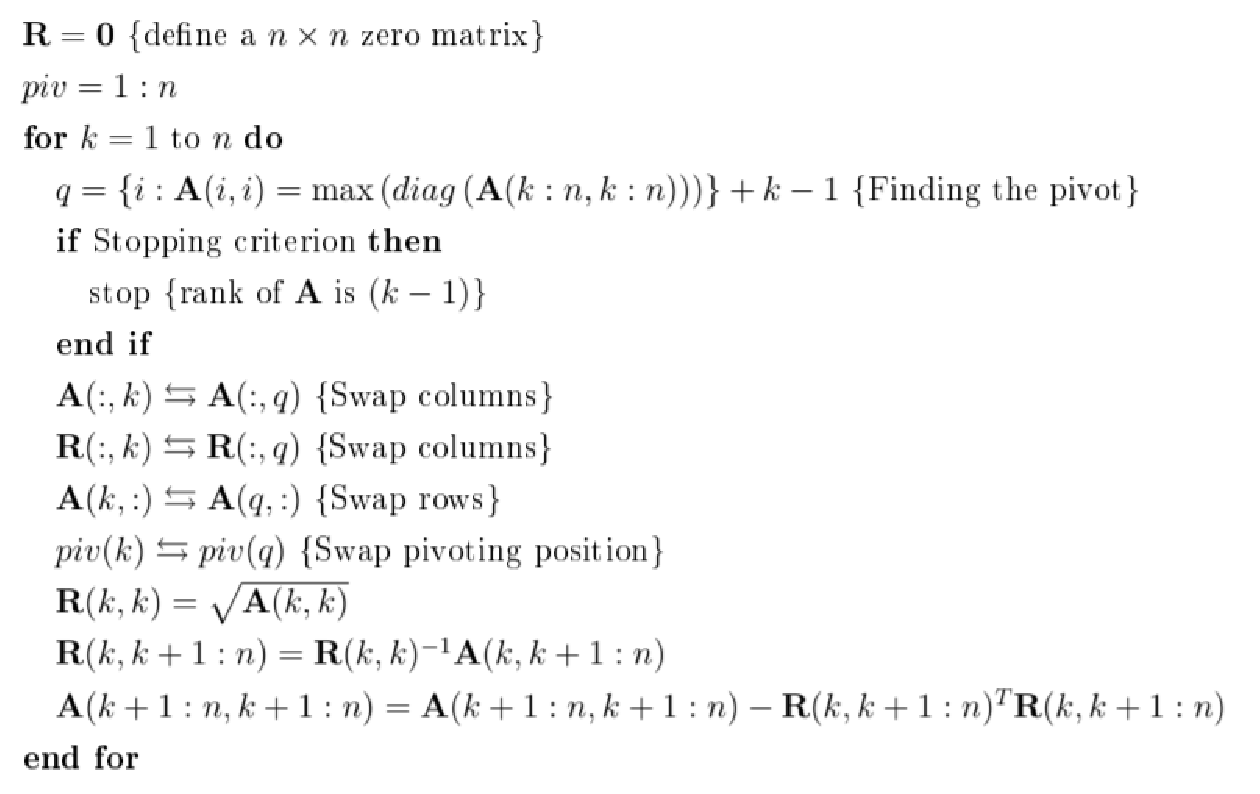
\includegraphics[width=0.6\textwidth]{PCC}
	\end{center}
	\caption{Pseudo-code for Pivoting Cholesky Decomposition}
	\label{fig1}
\end{figure}


\end{document} % NOTHING AFTER THIS LINE IS PART OF THE DOCUMENT
